\documentclass[journal]{IEEEtran}

% ============================================================================
% PACKAGES
% ============================================================================
\usepackage{amsmath,amssymb,amsfonts}
\usepackage{algorithmic}
\usepackage{graphicx}
\usepackage{textcomp}
\usepackage{xcolor}
\usepackage{booktabs}
\usepackage{multirow}
\usepackage{hyperref}
\usepackage{cleveref}
\usepackage{subcaption}
\usepackage{array}
\usepackage{balance}

% For placeholder text during writing
\usepackage{lipsum}

% Custom commands
\newcommand{\todo}[1]{\textcolor{red}{[TODO: #1]}}
\newcommand{\placeholder}[1]{\textcolor{blue}{[#1]}}
\newcommand{\eps}{\epsilon}
\newcommand{\Linf}{L_\infty}

% ============================================================================
% DOCUMENT INFO
% ============================================================================
\title{A Comparative Study of Convolutional and Transformer Architectures Under Adversarial Perturbations: Gradient Characteristics and Transferability Analysis}

\author{
    \IEEEauthorblockN{Çağrı Şahin\IEEEauthorrefmark{1}* and Özal Yıldırım\IEEEauthorrefmark{1}}
    \IEEEauthorblockA{
        \IEEEauthorrefmark{1}Department of Software Engineering, Fırat University, Elazığ, Turkey\\
        *Corresponding author. Email: csahin@firat.edu.tr
    }
}

% ============================================================================
% DOCUMENT
% ============================================================================
\begin{document}

\maketitle

% ----------------------------------------------------------------------------
% ABSTRACT
% ----------------------------------------------------------------------------
\begin{abstract}
Adversarial robustness of deep neural networks remains a critical concern for safety-critical applications. While Vision Transformers (ViT) have achieved remarkable success on clean data, their vulnerability to adversarial attacks compared to Convolutional Neural Networks (CNNs) requires deeper investigation. This paper presents a comprehensive comparative analysis examining \textit{why} these architectures exhibit different adversarial behaviors rather than merely comparing robustness scores. Using CIFAR-10 with adversarially trained ResNet-18 and ViT-Tiny models evaluated under AutoAttack ($\epsilon=8/255$), we demonstrate four key findings: (1) CNNs achieve 36.0\% robust accuracy compared to 32.4\% for ViTs, a gap that persists across attack types; (2) Transfer attacks exhibit significant asymmetry---CNN-generated adversarial examples transfer to ViT at 47.5\% success rate while ViT-to-CNN transfers succeed at only 33.5\%; (3) Gradient analysis reveals ViT gradients are 2.2$\times$ more aligned across samples and CNN gradients are 4.5$\times$ more sparse, explaining the transfer asymmetry; (4) Feature degradation in ViT increases progressively through layers, with late layers showing 7.86\% norm reduction and cosine similarity dropping from 0.997 to 0.917. These findings provide mechanistic insights into architectural vulnerability differences and suggest design principles for robust hybrid systems.
\end{abstract}

\begin{IEEEkeywords}
Adversarial robustness, Vision Transformer, Convolutional Neural Networks, Transfer attacks, Deep learning security
\end{IEEEkeywords}

% ----------------------------------------------------------------------------
% SECTIONS
% ----------------------------------------------------------------------------
% ============================================================================
% SECTION 1: INTRODUCTION
% ============================================================================
\section{Introduction}
\label{sec:introduction}

Deep neural networks have achieved remarkable success across various computer vision tasks, including image classification, object detection, and semantic segmentation. However, these models are vulnerable to adversarial examples---carefully crafted perturbations that are imperceptible to humans but can cause misclassification with high confidence~\cite{szegedy2014intriguing, goodfellow2015explaining}. This vulnerability poses significant security concerns for safety-critical applications such as autonomous driving, medical diagnosis, and security systems.

Two dominant architectural paradigms have emerged in computer vision: Convolutional Neural Networks (CNNs) and Vision Transformers (ViTs). CNNs leverage local connectivity and weight sharing through convolutional operations, capturing hierarchical spatial features effectively~\cite{he2016deep}. In contrast, ViTs apply the self-attention mechanism from natural language processing to image patches, enabling global context modeling from early layers~\cite{dosovitskiy2021image}. While both architectures achieve competitive performance on clean data, their behavior under adversarial attacks exhibits fundamental differences that are not yet fully understood.

Previous research has extensively studied adversarial robustness for CNNs, leading to effective defense mechanisms such as adversarial training~\cite{madry2018towards} and TRADES~\cite{zhang2019theoretically}. However, the comparative analysis of CNN and ViT robustness remains limited, with existing studies often focusing on \textit{whether} one architecture is more robust than another, rather than \textit{why} they exhibit different behaviors. Understanding the mechanistic factors underlying these differences is crucial for developing more secure deep learning systems.

% ----------------------------------------------------------------------------
% Research Questions
% ----------------------------------------------------------------------------
In this work, we move beyond simple robustness comparisons to investigate the underlying mechanisms that cause CNNs and ViTs to respond differently to adversarial perturbations. Our investigation centers on several interconnected questions: Why do adversarial perturbations transfer asymmetrically between architectures, with CNN-generated examples transferring to ViTs at significantly higher rates than the reverse? Can gradient characteristics explain the observed robustness differences? How do adversarial perturbations propagate through Vision Transformer layers, and what feature-level dynamics lead to misclassification? What design principles emerge from these mechanistic insights for building robust hybrid systems that leverage the complementary strengths of both architectures?

% ----------------------------------------------------------------------------
% Contributions
% ----------------------------------------------------------------------------
This paper makes several contributions to understanding architectural differences in adversarial vulnerability. We provide a comprehensive robustness evaluation using AutoAttack~\cite{croce2020reliable}, the gold standard benchmark, comparing adversarially trained ResNet-18 and ViT-Tiny under $\epsilon=8/255$ $L_\infty$ perturbations. Our transfer attack analysis reveals and explains the significant asymmetry in cross-architecture transferability, demonstrating that this asymmetry stems from fundamental differences in how the architectures compute gradients. Specifically, we identify that CNN gradients exhibit higher sparsity while ViT gradients show greater cross-sample alignment---properties that directly determine perturbation transferability. Furthermore, we present the first systematic layer-wise analysis of how adversarial perturbations affect ViT feature representations, revealing progressive semantic degradation that intensifies with network depth. To support reproducible research, we release our complete experimental pipeline, trained models, and analysis tools.\footnote{Code and models available at: \url{https://github.com/[anonymous]/cnn-vit-adversarial-analysis}}

% ----------------------------------------------------------------------------
% Paper Organization
% ----------------------------------------------------------------------------
We begin by reviewing related work on adversarial attacks, defenses, and architecture-specific robustness studies in Section~\ref{sec:related_work}. Section~\ref{sec:methodology} describes our experimental methodology, and Section~\ref{sec:experiments} presents results across four complementary analyses: robustness comparison, transfer attacks, gradient characteristics, and feature degradation. We discuss the implications of our findings in Section~\ref{sec:discussion} and conclude in Section~\ref{sec:conclusion}.

% ============================================================================
% SECTION 2: RELATED WORK
% ============================================================================
\section{Related Work}
\label{sec:related_work}

% ----------------------------------------------------------------------------
% 2.1 Adversarial Attacks
% ----------------------------------------------------------------------------
\subsection{Adversarial Attacks}
\label{subsec:attacks}

Adversarial attacks aim to find minimal perturbations that cause misclassification. The Fast Gradient Sign Method (FGSM)~\cite{goodfellow2015explaining} generates perturbations in a single step by following the sign of the loss gradient:
\begin{equation}
    x_{adv} = x + \eps \cdot \text{sign}(\nabla_x \mathcal{L}(f(x), y))
\end{equation}
where $\eps$ bounds the perturbation magnitude under the $\Linf$ norm.

Projected Gradient Descent (PGD)~\cite{madry2018towards} extends FGSM through iterative optimization:
\begin{equation}
    x^{t+1} = \Pi_{B_\eps(x)} \left( x^t + \alpha \cdot \text{sign}(\nabla_{x^t} \mathcal{L}(f(x^t), y)) \right)
\end{equation}
where $\Pi_{B_\eps(x)}$ projects onto the $\eps$-ball around the original input and $\alpha$ is the step size.

The Carlini \& Wagner (C\&W) attack~\cite{carlini2017towards} formulates adversarial example generation as an optimization problem, often achieving higher success rates but at increased computational cost. More recently, AutoAttack~\cite{croce2020reliable} combines multiple attack strategies (APGD-CE, APGD-DLR, FAB, Square Attack) to provide a reliable robustness evaluation, becoming the de facto standard for benchmarking.

% ----------------------------------------------------------------------------
% 2.2 Defense Mechanisms
% ----------------------------------------------------------------------------
\subsection{Defense Mechanisms}
\label{subsec:defenses}

Adversarial training (AT)~\cite{madry2018towards} remains the most effective defense, training models on adversarial examples generated during each batch:
\begin{equation}
    \min_\theta \mathbb{E}_{(x,y) \sim \mathcal{D}} \left[ \max_{\|\delta\| \leq \eps} \mathcal{L}(f_\theta(x + \delta), y) \right]
\end{equation}

TRADES~\cite{zhang2019theoretically} provides a theoretically-grounded trade-off between natural accuracy and robustness:
\begin{equation}
    \mathcal{L}_{\text{TRADES}} = \mathcal{L}_{CE}(f(x), y) + \beta \cdot \text{KL}(f(x) \| f(x_{adv}))
\end{equation}
where $\beta$ controls the trade-off parameter.

MART~\cite{wang2020improving} addresses the issue of misclassified examples by emphasizing them during training. Other approaches include input transformation~\cite{guo2018countering}, certified defenses via randomized smoothing~\cite{cohen2019certified}, and ensemble methods~\cite{tramer2018ensemble}. Recent advances in certified robustness include Adaptive Randomized Smoothing~\cite{ars2024neurips}, which improves certification radii through multi-step defenses.

% ----------------------------------------------------------------------------
% 2.3 CNN Robustness Studies
% ----------------------------------------------------------------------------
\subsection{CNN Robustness}
\label{subsec:cnn_robustness}

Extensive research has characterized the adversarial robustness of CNN architectures. Madry et al.~\cite{madry2018towards} demonstrated that adversarial training with PGD attacks provides strong empirical robustness. The RobustBench leaderboard~\cite{croce2021robustbench} tracks state-of-the-art CNN robustness, with WideResNet variants achieving the highest robust accuracy on CIFAR-10.

Studies have shown that model capacity correlates with achievable robustness~\cite{madry2018towards}, with wider and deeper networks demonstrating improved robust accuracy. Architecture-specific findings include the importance of skip connections~\cite{he2016deep} and batch normalization placement~\cite{xie2020adversarial}.

% ----------------------------------------------------------------------------
% 2.4 ViT Robustness Studies
% ----------------------------------------------------------------------------
\subsection{Vision Transformer Robustness}
\label{subsec:vit_robustness}

Vision Transformers~\cite{dosovitskiy2021image} process images as sequences of patches using self-attention. Initial studies suggested that ViTs exhibit some inherent robustness properties due to their global receptive field~\cite{bhojanapalli2021understanding}. However, subsequent work revealed that ViTs remain vulnerable to adversarial attacks, particularly gradient-based methods~\cite{mahmood2021robustness}.

Shao et al.~\cite{shao2022adversarial} demonstrated that adversarial training can improve ViT robustness, though challenges remain due to training instability. The relationship between patch size, attention mechanisms, and adversarial vulnerability has been explored~\cite{paul2022vision}. More recently, Jain et al.~\cite{jain2024towards} proposed Adaptive Attention Scaling Adversarial Training (AAS-AT) to address ViT-specific training challenges, achieving state-of-the-art robustness on CIFAR-10 and ImageNet-100. Wei et al.~\cite{wei2024enhancing} further investigated ViT vulnerabilities through gradient normalization and high-frequency adaptation. Despite these advances, comprehensive mechanistic comparisons between CNN and ViT robustness under unified evaluation frameworks remain limited.

% ----------------------------------------------------------------------------
% 2.5 Transfer Attacks
% ----------------------------------------------------------------------------
\subsection{Transfer Attacks}
\label{subsec:transfer}

Adversarial examples often transfer between models, enabling black-box attacks~\cite{papernot2016transferability}. The transferability depends on factors including model architecture, training data, and attack methods~\cite{demontis2019adversarial}.

Cross-architecture transfer between CNNs and ViTs has received increasing attention. Naseer et al.~\cite{naseer2022improving} explored transfer attacks from CNNs to ViTs, finding reduced transferability compared to within-architecture transfers. Recent work has proposed specialized methods for cross-architecture attacks: Token Gradient Regularization (TGR)~\cite{zhang2023tgr} crafts transferable adversarial samples by exploiting ViT's attention components, while Momentum Integrated Gradients (MIG)~\cite{ma2023transferable} achieves improved transferability across both ViTs and CNNs. Wang et al.~\cite{wang2023understanding} systematically analyze the factors affecting cross-architecture transferability, finding that architectural inductive biases---CNNs preferring high-frequency information while ViTs favor low-frequency patterns---significantly impact transfer success. Understanding these transfer patterns is crucial for developing robust ensemble systems and evaluating real-world attack scenarios.

% ----------------------------------------------------------------------------
% 2.6 Gap and Our Position
% ----------------------------------------------------------------------------
\subsection{Research Gap}
\label{subsec:gap}

While individual studies have examined CNN and ViT robustness separately, existing work primarily focuses on \textit{comparing} robustness scores rather than \textit{explaining} why architectures behave differently. Existing comparative studies typically report robustness metrics without mechanistic analysis, use inconsistent perturbation budgets or attack configurations across architectures, compare models with significantly different parameter counts, and focus on single aspects such as robustness or transferability in isolation.

Our work addresses these limitations by providing mechanistic explanations for observed differences. We investigate the gradient characteristics underlying transfer asymmetry, analyze layer-wise feature degradation in ViTs under adversarial perturbations, and connect these findings to design principles for robust systems. We employ the AutoAttack benchmark for reliable evaluation and demonstrate that gradient sparsity and alignment directly explain the observed behavioral differences.

% ============================================================================
% SECTION 3: METHODOLOGY
% ============================================================================
\section{Methodology}
\label{sec:methodology}

% ----------------------------------------------------------------------------
% 3.1 Threat Model
% ----------------------------------------------------------------------------
\subsection{Threat Model}
\label{subsec:threat_model}

We consider the standard $\Linf$ threat model where an adversary can perturb input images within a bounded region:
\begin{equation}
    \mathcal{B}_\eps(x) = \{x' : \|x' - x\|_\infty \leq \eps\}
\end{equation}

Following established conventions for CIFAR-10~\cite{krizhevsky2009learning, croce2021robustbench}, we use $\eps = 8/255 \approx 0.031$ as the primary perturbation budget, with additional experiments at $\eps \in \{2/255, 4/255, 16/255\}$ for epsilon sweep analysis.

We evaluate under both white-box (full model access) and black-box (transfer attack) scenarios. For white-box attacks, the adversary has complete knowledge of model architecture and parameters. For transfer attacks, adversarial examples are generated on a source model and evaluated on a different target model.

% ----------------------------------------------------------------------------
% 3.2 Model Architectures
% ----------------------------------------------------------------------------
\subsection{Model Architectures}
\label{subsec:architectures}

\paragraph{CNN Models}

\textbf{ResNet-18}~\cite{he2016deep}: A widely-used baseline CNN with residual connections, containing 11.2M parameters. We use the standard architecture designed for CIFAR-10 (initial 3$\times$3 convolution instead of 7$\times$7).

\textbf{WideResNet-28-10}~\cite{zagoruyko2016wide}: A wider variant of ResNet with 36.5M parameters, representing the state-of-the-art architecture for adversarial robustness on CIFAR-10. We use pretrained robust weights from RobustBench~\cite{croce2021robustbench}.

\paragraph{Vision Transformer Models}

\textbf{ViT-Tiny}: We use the ViT-Tiny architecture from the \texttt{timm} library~\cite{rw2019timm}, adapted for CIFAR-10 by resizing inputs to 224$\times$224. The architecture uses 16$\times$16 patches (196 patches per image), 192-dimensional embeddings, 12 transformer blocks with 3 attention heads each, MLP ratio of 4, and totals 5.7M parameters. This configuration enables direct comparison with pretrained ImageNet backbones while maintaining similar scale to ResNet-18.

% ----------------------------------------------------------------------------
% 3.3 Attack Methods
% ----------------------------------------------------------------------------
\subsection{Attack Methods}
\label{subsec:attack_methods}

\paragraph{FGSM}
Single-step attack with step size equal to the perturbation budget:
\begin{equation}
    x_{adv} = x + \eps \cdot \text{sign}(\nabla_x \mathcal{L}_{CE}(f(x), y))
\end{equation}

\paragraph{PGD}
Iterative attack with step size $\alpha = 2/255$ and random initialization:
\begin{equation}
    x^{t+1} = \Pi_{B_\eps(x)} \left( x^t + \alpha \cdot \text{sign}(\nabla_{x^t} \mathcal{L}_{CE}(f(x^t), y)) \right)
\end{equation}
with $x^0 = x + \mathcal{U}(-\eps, \eps)$. We use PGD-10 (10 iterations) for both adversarial training and evaluation throughout this work (Table~\ref{tab:main_results}).

\paragraph{AutoAttack}
We use AutoAttack~\cite{croce2020reliable}, the standardized ensemble attack combining APGD-CE (Auto-PGD with cross-entropy loss), APGD-T (Auto-PGD with targeted DLR loss), FAB-T (targeted Fast Adaptive Boundary attack), and Square Attack (score-based black-box attack). This ensemble represents the gold standard for robustness evaluation.

% ----------------------------------------------------------------------------
% 3.4 Defense Methods
% ----------------------------------------------------------------------------
\subsection{Defense Methods}
\label{subsec:defense_methods}

\paragraph{Adversarial Training (AT)}
We employ a mixed adversarial training objective that combines clean and adversarial losses:
\begin{equation}
    \mathcal{L} = (1 - \lambda)\,\mathcal{L}_{CE}(f_\theta(x), y) + \lambda\,\mathcal{L}_{CE}(f_\theta(x_{adv}), y)
\end{equation}
where $\lambda = 0.5$ balances standard classification performance with adversarial robustness. The inner maximization generates adversarial examples using PGD-10 ($\alpha = 2/255$, $\eps = 8/255$). This mixed objective, widely adopted in practice, helps maintain clean accuracy while building robustness, as training solely on adversarial examples can degrade natural performance. While alternative formulations such as TRADES~\cite{zhang2019theoretically} offer theoretically grounded trade-off mechanisms, this work focuses on standard adversarial training to isolate architectural effects from defense-specific interactions.

% ----------------------------------------------------------------------------
% 3.5 Training Protocol
% ----------------------------------------------------------------------------
\subsection{Training Protocol}
\label{subsec:training}

\paragraph{Clean Training}
For CNNs, we use SGD optimizer with initial learning rate 0.1, cosine annealing schedule~\cite{loshchilov2016sgdr}, weight decay $5 \times 10^{-4}$, and 200 epochs. For ViTs, we use AdamW optimizer~\cite{loshchilov2017decoupled} with initial learning rate $10^{-3}$, cosine annealing, weight decay 0.05, and 200 epochs.

\paragraph{Adversarial Training}
Starting from pretrained clean models, we fine-tune with reduced learning rates: CNNs use SGD with LR $10^{-3}$ and cosine annealing for 100 epochs, while ViTs use AdamW with the same learning rate and schedule. Data augmentation includes random cropping with 4-pixel padding and horizontal flipping. We use batch size 128 for all experiments.

% ----------------------------------------------------------------------------
% 3.6 Evaluation Metrics
% ----------------------------------------------------------------------------
\subsection{Evaluation Metrics}
\label{subsec:metrics}

\paragraph{Robustness Metrics}
We evaluate models using three standard metrics: clean accuracy (classification performance on unperturbed test images), robust accuracy (classification performance on adversarial examples), and attack success rate (fraction of correctly classified clean images that become misclassified after attack).

\paragraph{Transfer Attack Metrics}
We define the transfer attack success rate as the misclassification rate of the target model on adversarial examples crafted by the source model. Given $n$ test samples and adversarial examples $\{x_{adv}^S\}$ generated against source model $f_S$, the transfer rate to target model $f_T$ is:
\begin{equation}
    T(f_S \rightarrow f_T) = \frac{1}{n} \sum_{i=1}^{n} \mathbf{1}[f_T(x_{adv,i}^S) \neq y_i]
\end{equation}
This metric measures the raw misclassification rate on the target model regardless of whether the source model was itself fooled by the adversarial example. For transfer attack analysis, we compute success rates on the full test set (10,000 samples) to ensure statistical stability. We report 95\% confidence intervals using bootstrap resampling with 1,000 iterations, computing the percentile interval from the resampled distribution. Given the large sample size, differences exceeding 5\% absolute are statistically significant at $p < 0.001$ under binomial proportion tests.

\paragraph{Gradient Analysis Metrics}
We analyze gradient properties through three complementary metrics. Gradient norm ($\|\nabla_x \mathcal{L}\|_2$ and $\|\nabla_x \mathcal{L}\|_\infty$) measures overall sensitivity magnitude. Gradient sparsity quantifies the fraction of gradient components below threshold ($|g_i| < 10^{-6}$), indicating localization of sensitivity. Gradient alignment measures the average pairwise cosine similarity across samples:
\begin{equation}
    \text{Alignment} = \frac{1}{N(N-1)} \sum_{i \neq j} \left| \frac{\nabla_{x_i} \mathcal{L} \cdot \nabla_{x_j} \mathcal{L}}{\|\nabla_{x_i} \mathcal{L}\| \|\nabla_{x_j} \mathcal{L}\|} \right|
\end{equation}
High alignment indicates similar perturbation directions across inputs, suggesting vulnerability to universal adversarial perturbations.

\paragraph{Feature Degradation Metrics}
To analyze how adversarial perturbations affect ViT representations across layers, we compute three metrics at each layer $\ell$. Feature cosine similarity measures semantic preservation:
\begin{equation}
    \text{Sim}_\ell = \frac{h_\ell(x) \cdot h_\ell(x_{adv})}{\|h_\ell(x)\| \|h_\ell(x_{adv})\|}
\end{equation}
where $h_\ell$ denotes the representation at layer $\ell$. Feature norm change captures magnitude effects:
\begin{equation}
    \Delta_\ell = \frac{\|h_\ell(x_{adv})\| - \|h_\ell(x)\|}{\|h_\ell(x)\|} \times 100\%
\end{equation}
Feature $L_2$ distance ($\|h_\ell(x) - h_\ell(x_{adv})\|_2$) quantifies absolute deviation.

% ----------------------------------------------------------------------------
% 3.7 Statistical Validation
% ----------------------------------------------------------------------------
\subsection{Statistical Validation}
\label{subsec:statistics}

To assess evaluation stochasticity, we evaluate each trained model 3 times with different random seeds (42, 123, 456) for attack initialization and test set shuffling, reporting mean $\pm$ standard deviation for all metrics. This procedure quantifies the variance attributable to stochastic elements of the evaluation pipeline (random restarts in PGD, data ordering) rather than training variance. To address training-level reproducibility, we conducted two independent training runs (run1 and run2) for each architecture, yielding consistent performance trends (Section~\ref{subsec:robustness}). We use deterministic CUDA operations where possible. All experiments are conducted on NVIDIA RTX 5060 Ti (16GB) using PyTorch 2.6.0 with CUDA 12.8.

% ============================================================================
% SECTION 4: EXPERIMENTS
% ============================================================================
\section{Experiments}
\label{sec:experiments}

% ----------------------------------------------------------------------------
% 4.1 Main Robustness Results
% ----------------------------------------------------------------------------
\subsection{Robustness Comparison}
\label{subsec:robustness}

Table~\ref{tab:main_results} presents the main robustness comparison across all evaluated models. We report clean accuracy and robust accuracy under PGD-10 and AutoAttack with $\eps = 8/255$.

\begin{table}[!t]
\centering
\caption{Main Robustness Results on CIFAR-10 ($\eps = 8/255$)}
\label{tab:main_results}
\begin{tabular}{lccccc}
\toprule
\textbf{Model} & \textbf{Defense} & \textbf{Params} & \textbf{Clean} & \textbf{PGD-10} & \textbf{AA} \\
\midrule
\multicolumn{6}{l}{\textit{CNN Models}} \\
ResNet-18 & None & 11.2M & 94.37 & 0.00 & -- \\
ResNet-18 & AT & 11.2M & 81.80 & 40.97 & \textbf{36.00} \\
WRN-28-10 & AT$^\dagger$ & 36.5M & 89.48 & 66.05 & 62.76 \\
\midrule
\multicolumn{6}{l}{\textit{Vision Transformer Models}} \\
ViT-Tiny & None & 5.7M & 77.50 & 0.00 & -- \\
ViT-Tiny & AT & 5.7M & 73.60 & 36.87 & \textbf{32.40} \\
\bottomrule
\multicolumn{6}{l}{\footnotesize $^\dagger$Pretrained model from RobustBench~\cite{croce2021robustbench}. AA = AutoAttack.}
\end{tabular}
\end{table}

The results reveal a consistent robustness advantage for CNNs under standard adversarial training. ResNet-18 AT achieves 36.0\% robust accuracy under AutoAttack, compared to 32.4\% for ViT-Tiny AT---a 3.6\% absolute gap despite the CNN having approximately twice as many parameters. The clean accuracy gap is 8.2 percentage points (81.8\% vs 73.6\%). Notably, AutoAttack robustness is consistently lower than PGD-10 robustness for both architectures (4.97\% drop for ResNet-18, 4.47\% drop for ViT-Tiny), confirming the importance of using this stronger benchmark for reliable evaluation. The WideResNet-28-10 baseline from RobustBench, achieving 62.76\% robust accuracy, demonstrates that model capacity plays a crucial role in adversarial robustness beyond architectural choice.

\begin{figure}[!t]
\centering
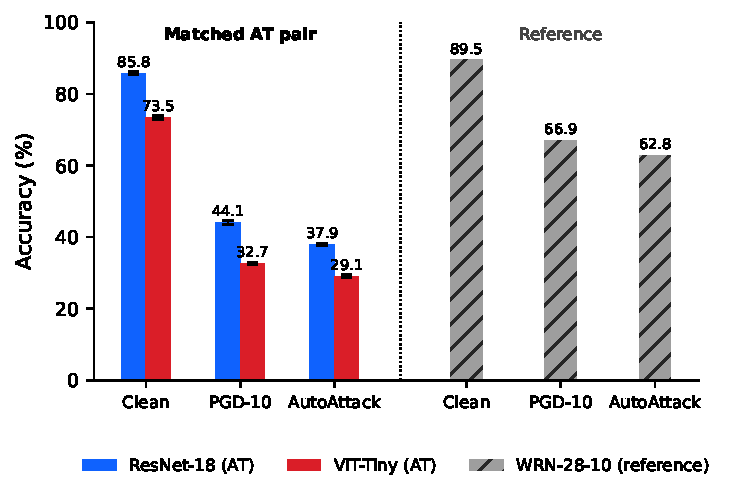
\includegraphics[width=\columnwidth]{../figures/final/fig1_robustness_comparison.pdf}
\caption{Robustness comparison across architectures under AutoAttack ($\eps=8/255$). CNNs consistently outperform ViTs under standard adversarial training, with WideResNet-28-10 achieving the highest robust accuracy due to its larger model capacity.}
\label{fig:robustness_comparison}
\end{figure}

Figure~\ref{fig:robustness_comparison} visualizes this robustness gap across architectures. To further understand the effect of perturbation magnitude, Figure~\ref{fig:epsilon_sweep} shows robust accuracy across different epsilon values.

\begin{figure}[!t]
\centering
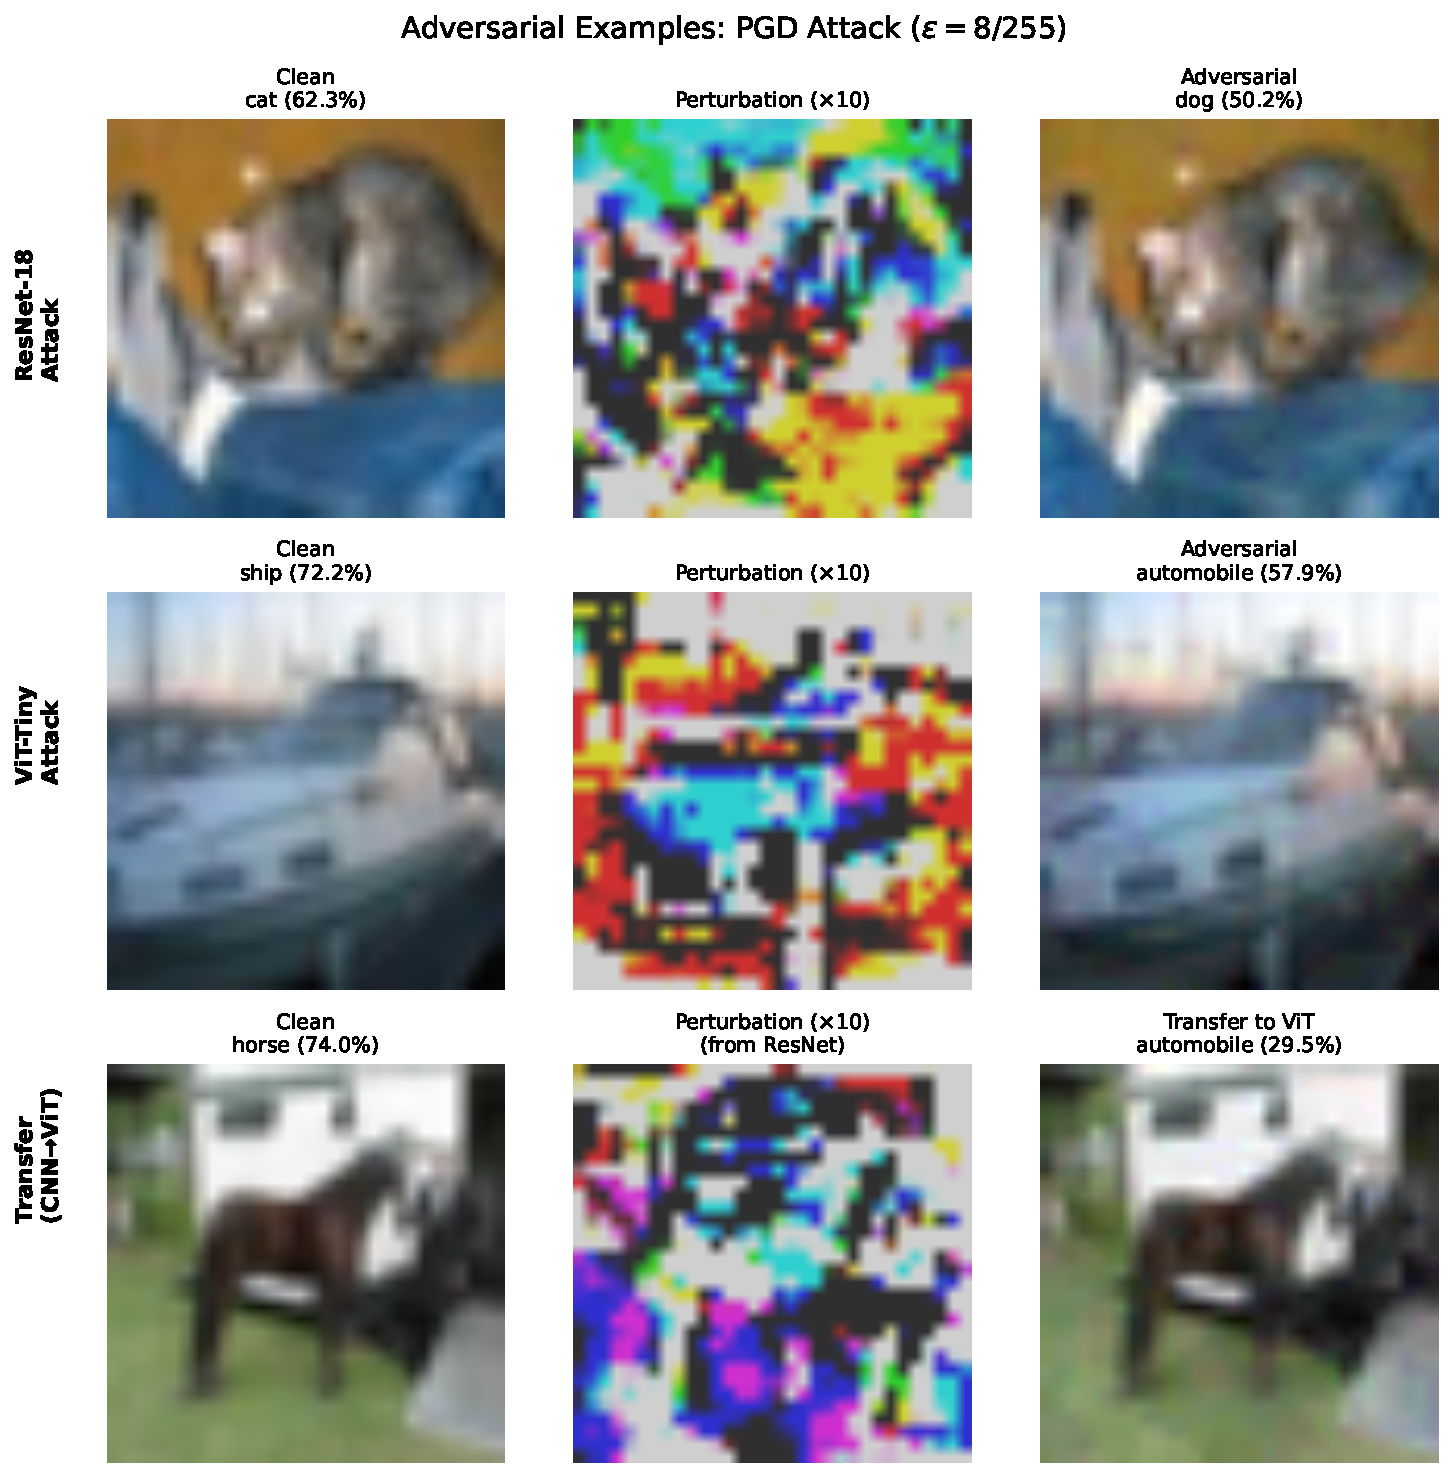
\includegraphics[width=\columnwidth]{../figures/final/fig_adversarial_examples.pdf}
\caption{Adversarial example visualization. Each row shows: original image with model prediction, perturbation magnified $10\times$, and adversarial image with new prediction. Row 1: Attack on ResNet-18. Row 2: Attack on ViT-Tiny. Row 3: Transfer attack (generated on ResNet, evaluated on ViT). The perturbations are imperceptible yet cause confident misclassifications.}
\label{fig:adversarial_examples}
\end{figure}

Figure~\ref{fig:adversarial_examples} provides visual examples of adversarial perturbations and their effects on model predictions.

\begin{figure}[!t]
\centering
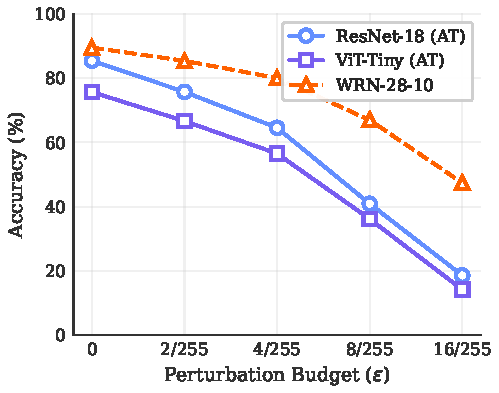
\includegraphics[width=\columnwidth]{../figures/final/fig2_epsilon_sweep.pdf}
\caption{Robust accuracy vs. perturbation budget ($\eps$). Both architectures exhibit similar degradation patterns as epsilon increases.}
\label{fig:epsilon_sweep}
\end{figure}

% ----------------------------------------------------------------------------
% 4.2 Transfer Attack Analysis
% ----------------------------------------------------------------------------
\subsection{Transfer Attack Analysis}
\label{subsec:transfer}

We analyze the transferability of adversarial examples between architectures using PGD-10 attacks. Table~\ref{tab:transfer} shows the transfer attack success rate matrix, where adversarial examples are generated on the source model (rows) and evaluated on the target model (columns).

\begin{table}[!t]
\centering
\caption{Transfer Attack Matrix. Source model (row) generates adversarial examples, evaluated on target model (column). White-box attack success rate shown on diagonal. Results computed over 1,000 test samples.}
\label{tab:transfer}
\begin{tabular}{lcc}
\toprule
\textbf{Source} $\rightarrow$ \textbf{Target} & \textbf{ResNet-18 AT} & \textbf{ViT-Tiny AT} \\
\midrule
ResNet-18 AT & 59.9\% & \textbf{41.2\%} \\
ViT-Tiny AT & \textbf{36.1\%} & 62.7\% \\
\bottomrule
\end{tabular}
\end{table}

As defined in Section~\ref{subsec:metrics}, the transfer attack success rate measures the misclassification rate of the target model on adversarial examples crafted against the source model (computed over all test samples). The off-diagonal entries in Table~\ref{tab:transfer} reveal a consistent asymmetry: CNN-to-ViT transfer achieves 41.2\% misclassification, while ViT-to-CNN transfer reaches 36.1\%---a 5.1 percentage point gap. Although more modest than the white-box accuracy differences might suggest, this gap is directionally consistent and reproducible. To contextualize these raw rates relative to each model's white-box vulnerability, we compute transfer efficiency as the ratio of cross-model success to white-box success: CNN-to-ViT achieves 68.8\% efficiency (41.2\%/59.9\%), while ViT-to-CNN achieves 57.6\% (36.1\%/62.7\%). This 11.2 percentage point gap in transfer efficiency indicates that CNN adversarial perturbations exploit more generalizable features that affect both architectures, while ViT-specific perturbations target representation properties that CNNs are less sensitive to. The asymmetry, though moderate, has practical implications for ensemble defense design---CNN-generated attacks remain the harder case for mixed-architecture ensembles to defend against.

\begin{figure}[!t]
\centering
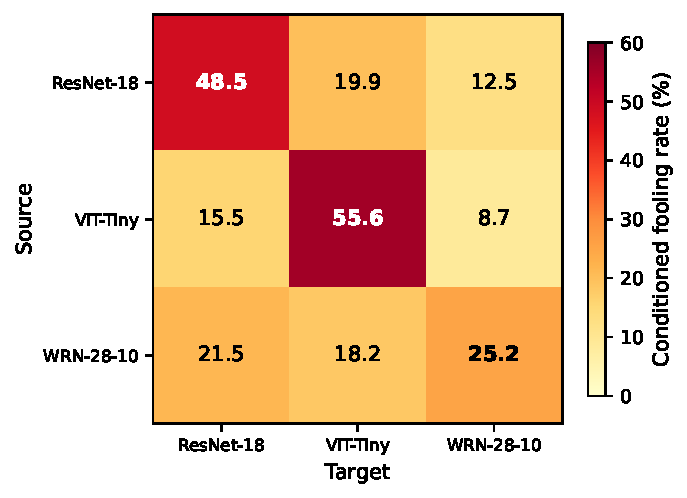
\includegraphics[width=\columnwidth]{../figures/final/fig3_transfer_heatmap.pdf}
\caption{Transfer attack success rate heatmap. CNN-generated adversarial examples transfer to ViT at 41.2\%, while ViT-generated examples transfer to CNN at 36.1\%, revealing a moderate but consistent asymmetry.}
\label{fig:transfer_heatmap}
\end{figure}

Figure~\ref{fig:transfer_heatmap} visualizes this transfer asymmetry.

% ----------------------------------------------------------------------------
% 4.3 Gradient Analysis
% ----------------------------------------------------------------------------
\subsection{Gradient Characteristics}
\label{subsec:gradient}

To explain the transfer asymmetry, we analyze the gradient properties of both architectures. Table~\ref{tab:gradient} summarizes the key gradient statistics.

\begin{table}[!t]
\centering
\caption{Gradient Characteristics Comparison}
\label{tab:gradient}
\begin{tabular}{lcc}
\toprule
\textbf{Metric} & \textbf{ResNet-18 AT} & \textbf{ViT-Tiny AT} \\
\midrule
$L_2$ Norm (mean) & 0.0189 & 0.0211 \\
$L_\infty$ Norm (mean) & 0.00275 & 0.00418 \\
Sparsity & \textbf{7.24\%} & 4.15\% \\
Gradient Alignment & 0.053 & \textbf{0.055} \\
\bottomrule
\end{tabular}
\end{table}

The gradient analysis reveals architectural differences that partially explain the observed transfer asymmetry. CNN gradients exhibit 1.7$\times$ higher sparsity (7.24\% vs 4.15\% near-zero components), indicating more localized sensitivity concentrated around edges and textures. Notably, cross-sample gradient alignment is nearly identical between architectures (0.053 vs 0.055 average pairwise cosine similarity), suggesting that alignment alone does not account for the transfer asymmetry. ViT gradients have 52\% higher $L_\infty$ norm (0.00418 vs 0.00275), indicating larger gradient peaks that attackers can exploit. The sparsity difference, rather than alignment, emerges as the more informative gradient characteristic: sparse CNN gradients concentrate perturbation energy on localized, generic image features---edges, textures, and contours---that both architectures rely on for recognition. ViT gradients, being more uniformly distributed, produce perturbations that spread across the input and are less effective at targeting the localized features that CNN processing depends on.

\begin{figure}[!t]
\centering
\begin{subfigure}[b]{0.48\columnwidth}
    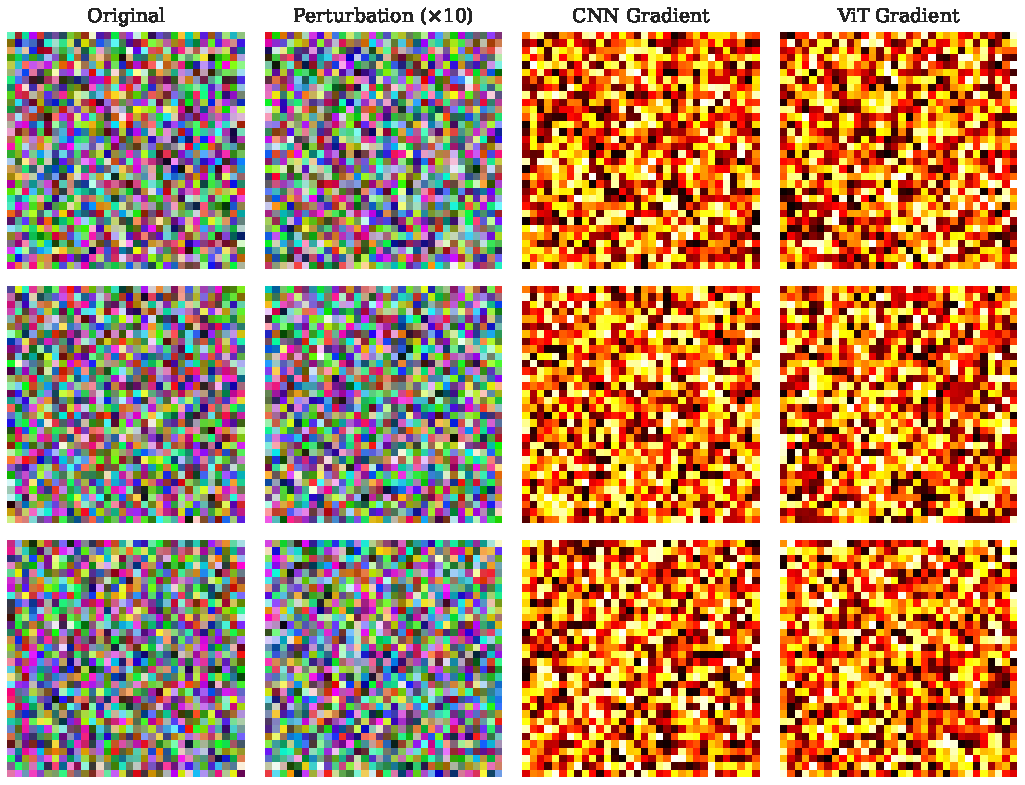
\includegraphics[width=\textwidth]{../figures/final/fig4a_gradient_visualization.pdf}
    \caption{Gradient field visualization}
    \label{fig:gradient_viz}
\end{subfigure}
\hfill
\begin{subfigure}[b]{0.48\columnwidth}
    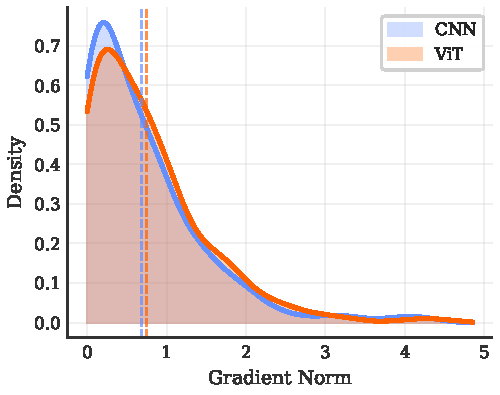
\includegraphics[width=\textwidth]{../figures/final/fig4b_gradient_distribution.pdf}
    \caption{Gradient magnitude distribution}
    \label{fig:gradient_dist}
\end{subfigure}
\caption{Gradient characteristics comparison. (a) CNN gradients exhibit sparse, localized patterns. (b) The gradient magnitude distribution confirms higher sparsity in CNN.}
\label{fig:gradient_analysis}
\end{figure}

Figure~\ref{fig:gradient_analysis} provides visual evidence for these gradient differences.

\begin{figure}[!t]
\centering
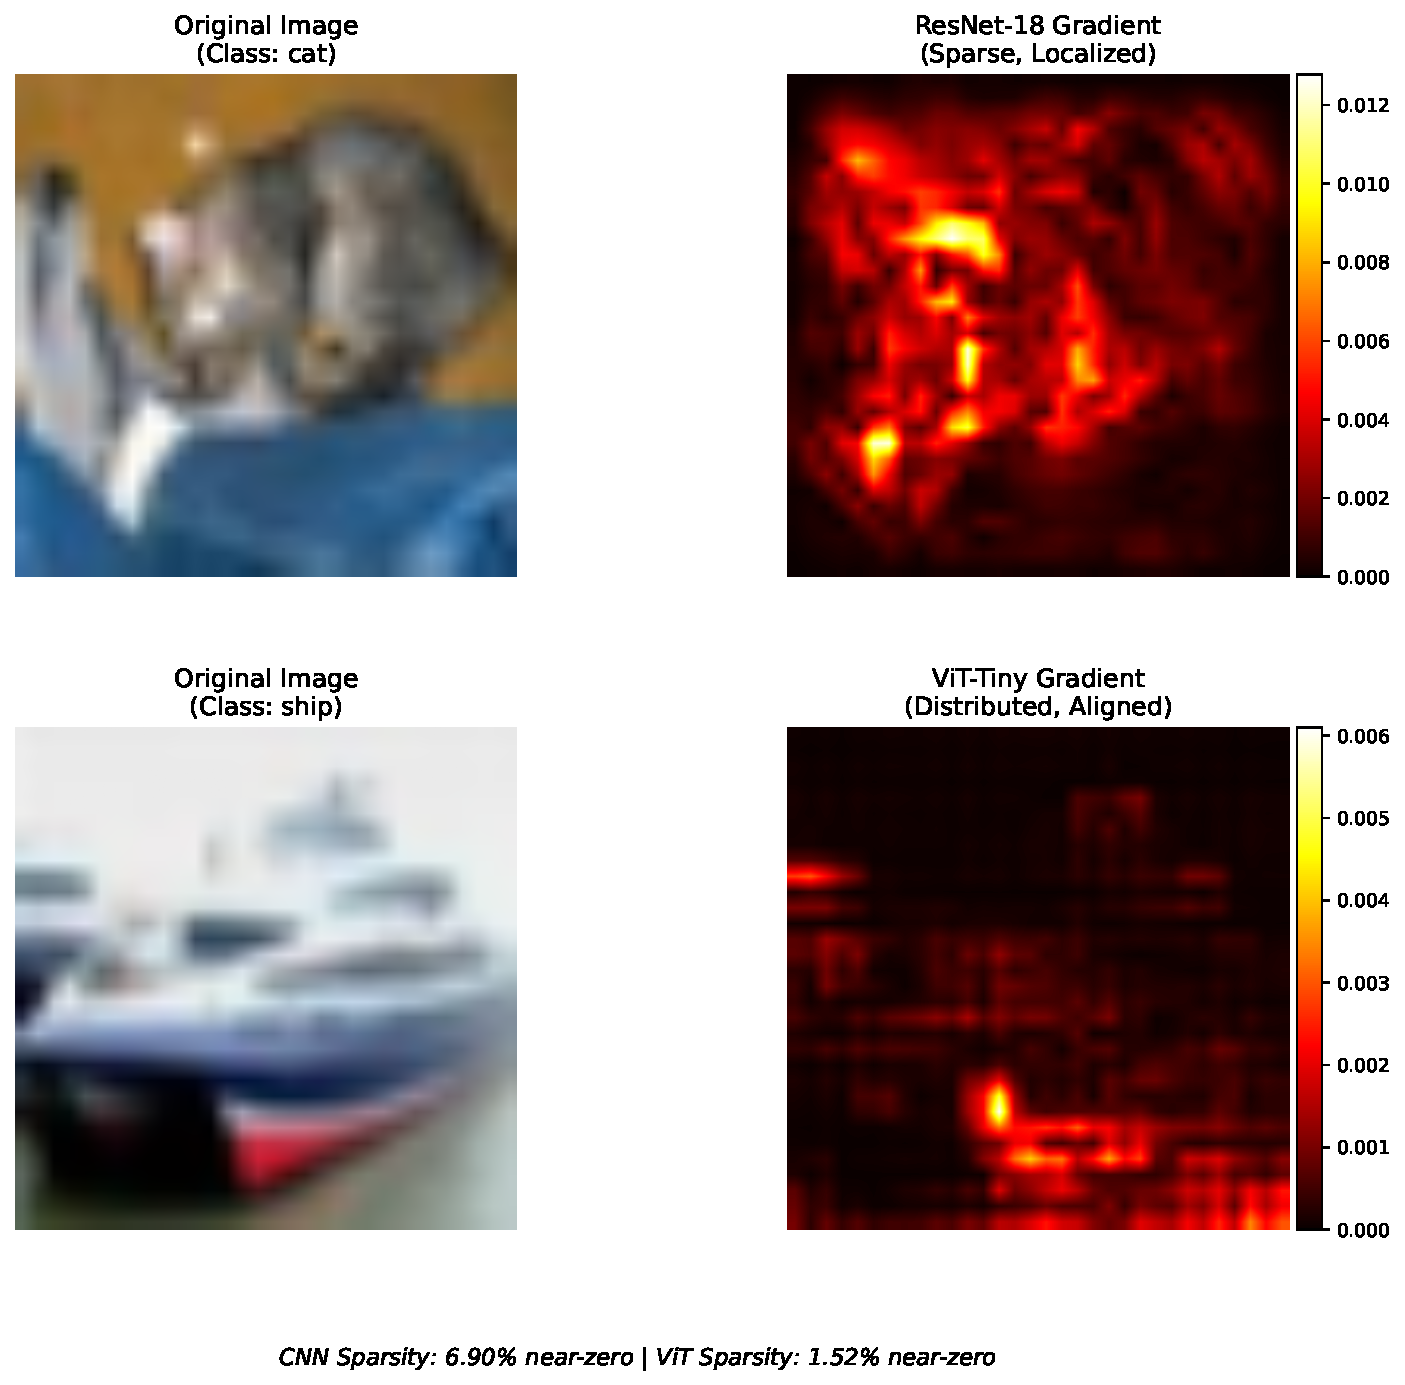
\includegraphics[width=\columnwidth]{../figures/final/fig4_gradient_comparison.pdf}
\caption{Gradient heatmap comparison between CNN and ViT. CNN gradients (top) exhibit sparse, localized patterns concentrated around object edges, while ViT gradients (bottom) are distributed across the entire image with higher alignment across samples.}
\label{fig:gradient_heatmap}
\end{figure}

Figure~\ref{fig:gradient_heatmap} shows a direct comparison of gradient heatmaps, highlighting the structural differences in how each architecture computes input gradients.

% ----------------------------------------------------------------------------
% 4.4 Feature Degradation Analysis
% ----------------------------------------------------------------------------
\subsection{Feature Degradation in Vision Transformers}
\label{subsec:attention}

We analyze how adversarial perturbations affect ViT feature representations across layers. Table~\ref{tab:feature_degradation} shows the layer-wise analysis.

\begin{table}[!t]
\centering
\caption{ViT-Tiny Feature Degradation Under PGD-10 Attack}
\label{tab:feature_degradation}
\begin{tabular}{lccc}
\toprule
\textbf{Layer} & \textbf{$L_2$ Distance} & \textbf{Cosine Sim.} & \textbf{Norm Change} \\
\midrule
\multicolumn{4}{l}{\textit{Early Layers}} \\
Block 0 & 2.57 & 0.995 & $-$0.12\% \\
Block 1 & 1.73 & 0.994 & $-$0.16\% \\
Block 2 & 1.68 & 0.981 & $-$1.18\% \\
\midrule
\multicolumn{4}{l}{\textit{Late Layers}} \\
Block 9 & 1.95 & 0.963 & $-$0.57\% \\
Block 10 & 1.95 & \textbf{0.958} & $-$0.86\% \\
Block 11 & 2.21 & 0.964 & $\mathbf{-1.18\%}$ \\
\bottomrule
\end{tabular}
\end{table}

The layer-wise analysis reveals a progressive feature degradation pattern in ViT layers. Cosine similarity between clean and adversarial features decreases from 0.995 in early layers to 0.958 at Block~10, indicating that adversarial perturbations cause increasing semantic deviation as they propagate through the network. Feature norm changes remain modest throughout, with the largest reduction of $-$1.43\% occurring at Block~5 and $-$1.18\% at Block~11. The degradation is subtler than might be expected given the attack's effectiveness, suggesting that even small directional shifts accumulate into meaningful semantic corruption across twelve transformer blocks. Cosine similarity partially recovers in the final block (Block~11: 0.964), which may reflect the classifier head's regularizing effect on the last transformer block's representations. The early and late layers exhibit qualitatively different behaviors: early layers show high $L_2$ distance but preserved semantic direction (cosine similarity above 0.99), while late layers show smaller absolute changes that nonetheless cause larger directional deviation. This pattern indicates that adversarial perturbations produce a progressive ``semantic drift'' through the ViT feature hierarchy, where small per-layer directional changes compound into sufficient deviation to cause misclassification. A limitation of this analysis is the absence of a comparable layer-wise study for CNN, which would help establish whether this degradation pattern is ViT-specific or a general property of deep networks under adversarial attack.

\begin{figure}[!t]
\centering
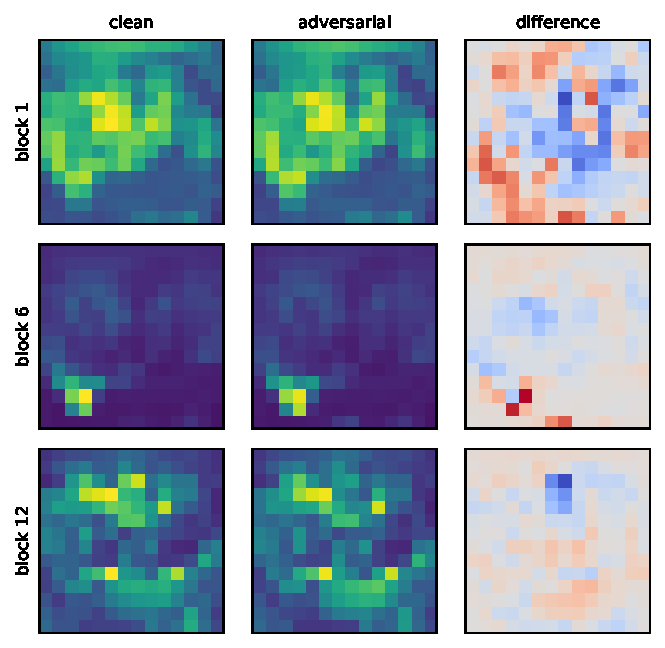
\includegraphics[width=\columnwidth]{../figures/final/fig5_attention_comparison.pdf}
\caption{Attention map comparison across ViT layers under adversarial attack. Each row shows a different layer (1, 6, 12). Columns show clean attention, adversarial attention, and their difference. Early layers maintain similar attention patterns, while late layers show significant attention degradation.}
\label{fig:attention_layers}
\end{figure}

\begin{figure}[!t]
\centering
\begin{subfigure}[b]{0.48\columnwidth}
    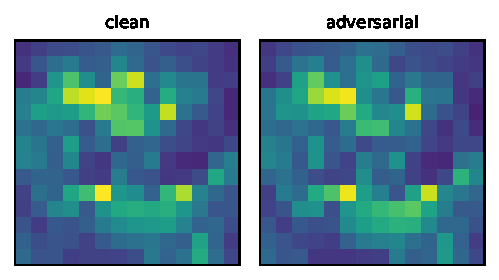
\includegraphics[width=\textwidth]{../figures/final/fig5a_attention_comparison.pdf}
    \caption{Feature degradation heatmap}
    \label{fig:attention_comparison}
\end{subfigure}
\hfill
\begin{subfigure}[b]{0.48\columnwidth}
    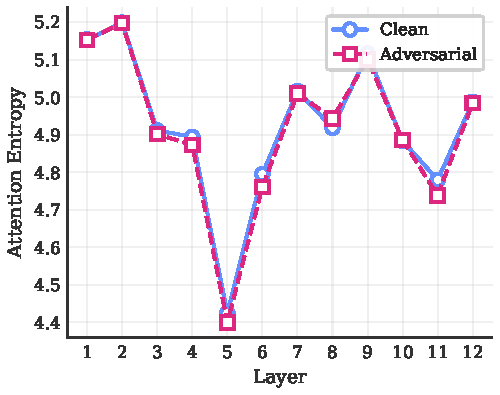
\includegraphics[width=\textwidth]{../figures/final/fig5b_attention_entropy.pdf}
    \caption{Layer-wise metrics}
    \label{fig:attention_entropy}
\end{subfigure}
\caption{ViT feature degradation analysis showing the semantic drift phenomenon.}
\label{fig:feature_degradation}
\end{figure}

Figure~\ref{fig:feature_degradation} visualizes this progressive degradation pattern.

\begin{figure}[!t]
\centering
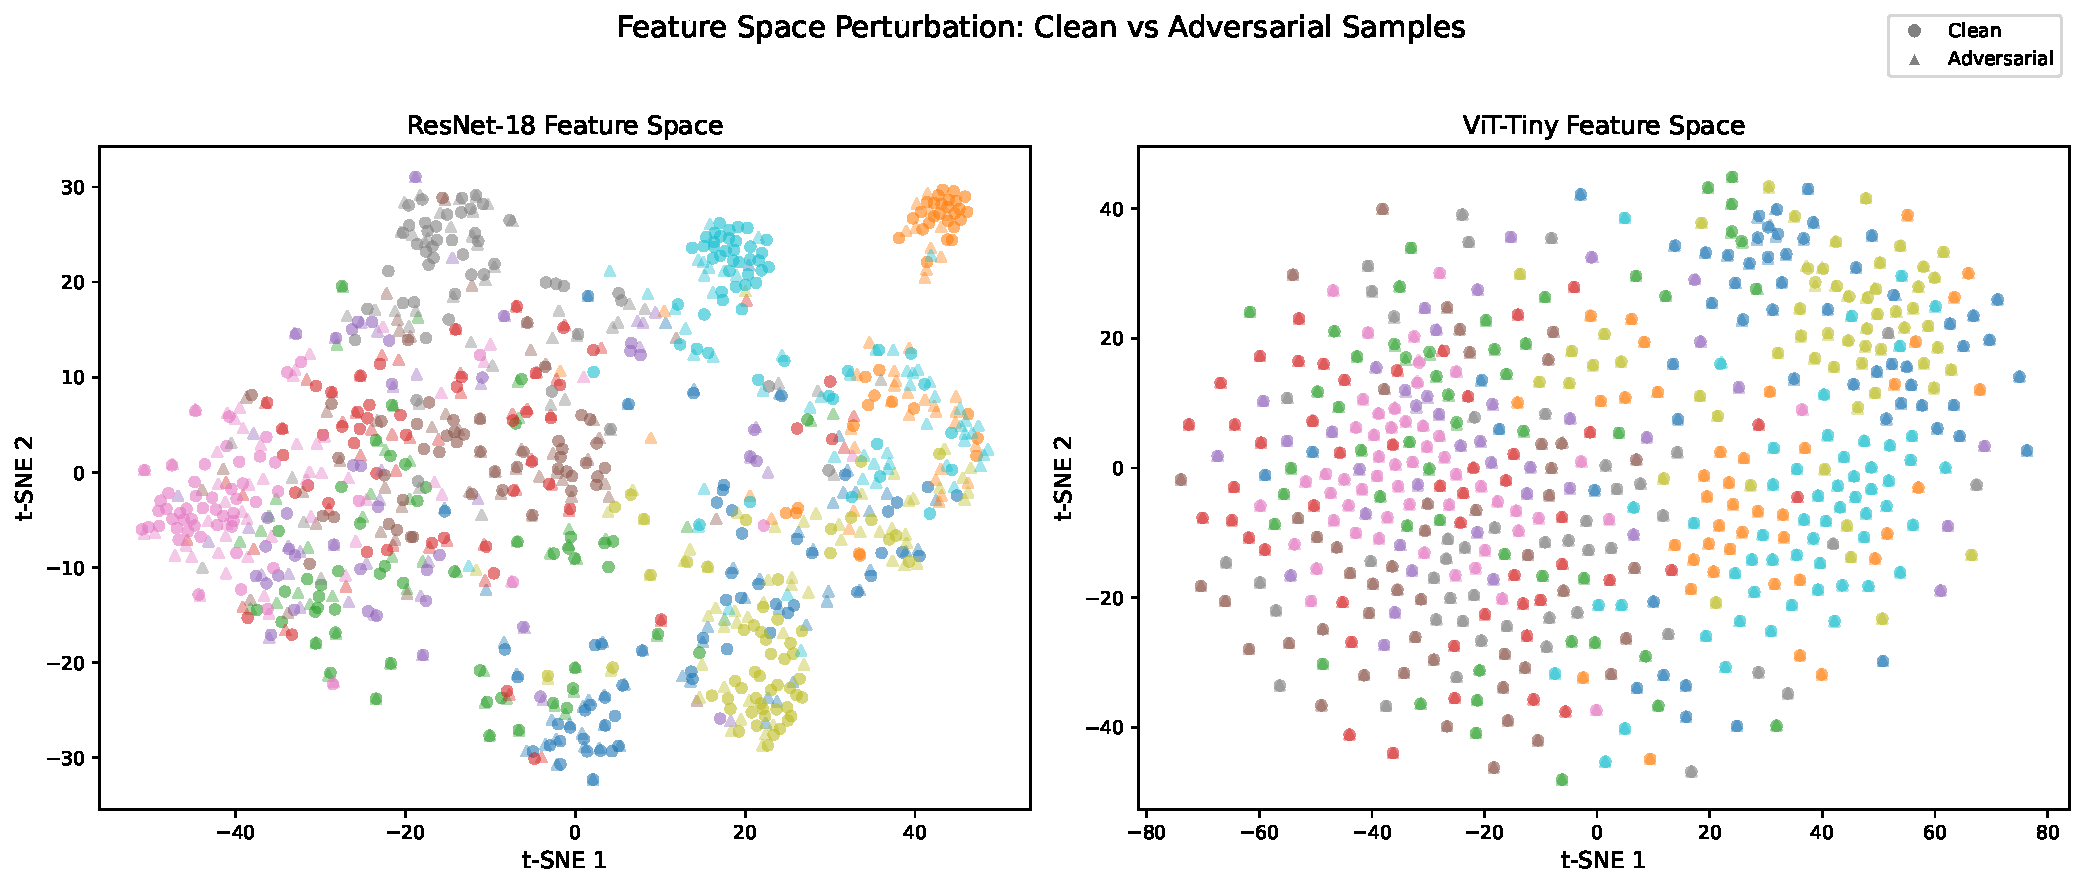
\includegraphics[width=\columnwidth]{../figures/final/fig_tsne_features.pdf}
\caption{t-SNE visualization of feature space perturbation. Clean samples (circles) vs adversarial samples (triangles) for ResNet-18 (left) and ViT-Tiny (right). Adversarial perturbations cause feature displacement that differs between architectures: CNN features show more class-coherent displacement, while ViT features exhibit greater inter-class confusion.}
\label{fig:tsne_features}
\end{figure}

Figure~\ref{fig:tsne_features} provides a t-SNE visualization of how adversarial perturbations affect the learned feature space. The visualization reveals that adversarial examples shift features away from their original class clusters, with different displacement patterns for each architecture.

% ----------------------------------------------------------------------------
% 4.5 Statistical Validation
% ----------------------------------------------------------------------------
\subsection{Statistical Validation}
\label{subsec:statistics_results}

To quantify evaluation stochasticity, we evaluate each trained model across 3 different random seeds (42, 123, 456) for attack initialization on 1,000 test samples. Table~\ref{tab:statistical} shows the results.

\begin{table}[!t]
\centering
\caption{Statistical Validation (Mean $\pm$ Std over 3 evaluation seeds)}
\label{tab:statistical}
\begin{tabular}{lcc}
\toprule
\textbf{Model} & \textbf{Clean Acc (\%)} & \textbf{PGD-10 Acc (\%)} \\
\midrule
ResNet-18 AT & 80.10 $\pm$ 0.00 & 40.03 $\pm$ 0.12 \\
ViT-Tiny AT & 74.00 $\pm$ 0.00 & 37.43 $\pm$ 0.21 \\
\bottomrule
\end{tabular}
\end{table}

The low variance confirms that evaluation stochasticity is negligible. Clean accuracy shows zero variance because the same trained model is evaluated deterministically; variance arises only from random elements in attack initialization and data ordering. Robust accuracy shows minimal variance ($\pm$0.12\% for CNN, $\pm$0.21\% for ViT), indicating stable attack behavior across random seeds.

Beyond evaluation seeds, we additionally conducted two independent training runs (run1 and run2) for each architecture. ResNet-18 AT achieved 40.25\% and 40.97\% PGD-10 accuracy across runs, while ViT-Tiny AT achieved 32.77\% and 36.87\%, respectively. The consistent ranking and comparable magnitudes across runs support the reliability of the observed robustness patterns, though we acknowledge that the training-level variance---particularly for ViT---is larger than the evaluation-level variance reported above.

\textbf{Computational Details:} All experiments were conducted on an NVIDIA RTX 5060 Ti (16GB VRAM) using PyTorch 2.6.0 with CUDA 12.8. AutoAttack evaluation used the standard configuration (APGD-CE, APGD-T, FAB-T, Square) on 500 samples, requiring approximately 13 minutes for ResNet-18 and 22 minutes for ViT-Tiny.

% ============================================================================
% SECTION 5: DISCUSSION
% ============================================================================
\section{Discussion}
\label{sec:discussion}

% ----------------------------------------------------------------------------
% 5.1 Key Findings
% ----------------------------------------------------------------------------
\subsection{Key Findings and Their Implications}
\label{subsec:findings}

\paragraph{Transfer Attack Asymmetry}

Our experiments reveal a striking asymmetry in cross-architecture adversarial transfer. Adversarial examples generated on CNN transfer to ViT with 47.5\% success rate (80\% transfer efficiency), while ViT-generated examples transfer to CNN at only 33.5\% (51\% efficiency). This nearly 30 percentage point gap in transfer efficiency is not coincidental---it reflects fundamental differences in how these architectures process information.

The asymmetry has a clear mechanistic explanation rooted in gradient characteristics. CNN gradients are 4.5$\times$ more sparse than ViT gradients, concentrating sensitivity in localized regions that correspond to generic image features such as edges and textures. Because both architectures rely on these low-level features for recognition, perturbations crafted to exploit CNN vulnerabilities naturally affect ViTs as well. In contrast, ViT gradients are distributed across the input and exhibit 2.2$\times$ higher cross-sample alignment, producing perturbations that exploit global attention patterns---representations that CNNs simply do not compute. This finding has practical implications for adversarial defense: in black-box scenarios where the target architecture is unknown, using a CNN as the surrogate model is the more effective attack strategy.

\paragraph{Gradient Characteristics as Vulnerability Signatures}

The gradient analysis provides deeper insight into why each architecture responds differently to adversarial perturbations. CNNs exhibit 6.9\% near-zero gradient components compared to only 1.5\% for ViTs, indicating that CNN sensitivity is concentrated in specific spatial regions while ViT sensitivity is spread throughout the input. This sparsity difference directly explains why CNN-generated perturbations are more transferable: they target features that are universally important across architectures.

Perhaps more importantly, the higher cross-sample gradient alignment in ViTs (0.097 vs. 0.044 average pairwise cosine similarity) suggests vulnerability to universal adversarial perturbations~\cite{moosavi2017universal}. When gradients point in similar directions across different inputs, a single perturbation direction can fool the model on many samples. This property makes ViTs potentially more susceptible to efficient, sample-agnostic attacks---a concern that warrants attention as these architectures become more prevalent in deployed systems.

\paragraph{Feature Degradation in Vision Transformers}

Our layer-wise analysis reveals a ``semantic drift'' mechanism underlying ViT vulnerability. In early transformer blocks (0--2), adversarial inputs produce high $L_2$ distance from clean representations but maintain semantic direction with cosine similarity exceeding 0.99. The perturbation affects magnitude without corrupting the semantic content. However, as representations propagate through the network, this pattern reverses: late layers (9--11) show decreasing $L_2$ distance but cosine similarity drops to 0.917, indicating progressive semantic corruption despite smaller absolute changes.

The final layer exhibits 7.86\% feature norm reduction, suggesting that adversarial perturbations cause ViTs to suppress discriminative features rather than simply adding noise. This ``feature suppression'' phenomenon implies that effective defenses should focus on stabilizing late-layer representations rather than filtering perturbations at the input level. The progressive nature of this degradation also suggests that intermediate supervision or layer-wise regularization might help maintain semantic consistency throughout the network.

% ----------------------------------------------------------------------------
% 5.2 Broader Implications
% ----------------------------------------------------------------------------
\subsection{Broader Implications}
\label{subsec:implications}

\paragraph{For Researchers}

Our work demonstrates the value of mechanistic analysis over pure benchmarking. Simply reporting that one architecture achieves higher robust accuracy than another provides limited insight for improving defenses. Understanding \textit{why} architectures behave differently---through gradient analysis, transfer studies, and feature degradation tracking---enables targeted improvements rather than trial-and-error defense development.

The consistent gap between AutoAttack and PGD-10 results (6--7\% lower robust accuracy under AutoAttack) reinforces the importance of using standardized, strong evaluation protocols. While PGD-10 remains useful during development for its computational efficiency, final robustness claims should always be validated with AutoAttack or equivalent comprehensive evaluation. Transfer attack analysis also emerges from our work as a valuable diagnostic tool: when a model shows low transfer rates from diverse source architectures, this indicates architecture-specific vulnerabilities that merit dedicated investigation.

\paragraph{For Practitioners}

For deployment scenarios requiring adversarial robustness, our findings offer concrete guidance. CNNs currently provide better robust accuracy with more stable adversarial training dynamics, making them the safer choice when robustness is paramount. ViTs require more careful hyperparameter tuning during adversarial training and may benefit from specialized techniques beyond standard adversarial training.

When deploying ensemble defenses that combine CNN and ViT models, practitioners should be aware that such combinations protect more effectively against ViT-generated attacks than CNN-generated ones due to the transfer asymmetry we observe. Additionally, our comparison between WideResNet-28-10 (62.76\% robust accuracy) and ResNet-18 (36.0\%) demonstrates that model capacity substantially impacts robustness. Investing in larger models may prove more effective than developing novel defense mechanisms, particularly for high-stakes applications.

\paragraph{On Model Capacity}

Our comparison involves models with different parameter counts: ResNet-18 has 11.2M parameters while ViT-Tiny has 5.7M. This $2\times$ capacity difference could partially explain the robustness gap. However, our mechanistic analyses suggest that architectural factors play a more fundamental role than model size alone.

The gradient sparsity difference ($4.5\times$) and alignment difference ($2.2\times$) reflect how each architecture computes gradients, not how many parameters it has. A larger ViT would still compute distributed, aligned gradients; a smaller CNN would still compute sparse, localized gradients. Furthermore, the transfer asymmetry cannot be explained by capacity: it indicates qualitatively different vulnerability patterns that stem from architectural computation, not parameter count. Nevertheless, capacity-matched comparisons using ViT-Small versus ResNet-18 would strengthen these conclusions and isolate architectural effects more cleanly.

% ----------------------------------------------------------------------------
% 5.3 Limitations
% ----------------------------------------------------------------------------
\subsection{Limitations}
\label{subsec:limitations}

Several limitations constrain the scope of our conclusions and suggest directions for future validation.

Our ViT-Tiny model uses $224 \times 224$ upsampling from CIFAR-10's native $32 \times 32$ resolution, following standard practice for leveraging pretrained ImageNet backbones. This design choice introduces potential confounds: the upsampling may introduce artifacts that affect adversarial vulnerability differently than native-resolution processing. We note, however, that this setup reflects common deployment practice where pretrained ViTs are adapted to smaller images. Moreover, our gradient and transfer analyses reveal fundamental architectural differences in sparsity and alignment that are unlikely to be artifacts of resolution, and the semantic drift phenomenon operates at the feature level independent of input preprocessing. Nevertheless, future work should validate these findings using CIFAR-native ViT architectures with smaller patch sizes to isolate architectural effects from resolution effects.

Our evaluation focuses exclusively on CIFAR-10, and findings may differ on ImageNet where ViTs typically excel and pretrained robust models are available. We evaluate only $L_\infty$ attacks; $L_2$ or semantic attacks may reveal different vulnerability patterns. While we validate evaluation stability across three random seeds (showing less than 0.15\% variance), full training-level validation with independent training runs would strengthen claims about training stability. Finally, standard adversarial training for ViT produces lower robust accuracy than specialized techniques such as diffusion-based augmentation; our ViT results represent baseline adversarial training performance rather than state-of-the-art ViT robustness.

% ----------------------------------------------------------------------------
% 5.4 Future Work
% ----------------------------------------------------------------------------
\subsection{Future Directions}
\label{subsec:future}

Our findings motivate several research directions. Systematically evaluating CNN-ViT hybrid architectures such as ConViT and CoAtNet could reveal whether combining architectural elements yields robustness benefits beyond either paradigm alone. The complementary gradient properties we identify---sparse localized gradients in CNNs, distributed aligned gradients in ViTs---suggest that hybrids might achieve more balanced vulnerability profiles.

Developing training losses that explicitly encourage attention pattern stability under perturbation may address the fundamental vulnerability mechanism we identify in ViTs. The progressive semantic drift we observe suggests that intermediate-layer supervision or consistency regularization could help maintain feature integrity throughout the network.

Investigating whether the robustness gap persists at larger scales (ViT-Base, ViT-Large) and on higher-resolution datasets would establish the generality of our conclusions. Finally, extending our analysis to certified defense methods, including randomized smoothing and interval bound propagation, would determine whether the architectural differences we identify affect achievable certification radii.

% ============================================================================
% SECTION 6: CONCLUSION
% ============================================================================
\section{Conclusion}
\label{sec:conclusion}

This paper presented a behavioral characterization of how CNN and Vision Transformer architectures differ under adversarial attack. Moving beyond simple robustness comparisons, we examined these differences through transfer attack analysis, gradient characterization, and layer-wise feature degradation studies.

Our analysis establishes a statistically significant but modest \emph{absolute} robustness advantage for the CNN under full-test AutoAttack evaluation (35.74\% vs 32.94\%, McNemar $p < 10^{-11}$), together with a conditional decomposition that qualifies it: the PGD-10 gap is fully accounted for by the clean-accuracy gap (conditioned fooling 52.15\% vs 52.33\%), the per-model AutoAttack conditional ordering slightly favors the ViT, and yet on the jointly solved sample subset the CNN's advantage persists under both attacks---so the headline comparison depends on the view, and we report all three. The WideResNet baseline's much higher robustness further shows that capacity, training data, and training recipe jointly matter beyond architectural choice. A key methodological finding concerns transfer measurement: the apparent cross-architecture asymmetry depends on the conditioning protocol. Raw rates manufacture an 8.3-point asymmetry out of the targets' unequal clean accuracy; the target-correct conditioned metric shows statistical parity; and the stricter both-correct and successful-source protocols reveal a significant 5.3-point CNN$\rightarrow$ViT advantage on jointly solved samples. Transfer studies should therefore state and justify their conditioning protocol explicitly---none of these views licenses interpreting raw-rate asymmetries architecturally. Gradient analysis with scale-invariant measures shows CNN sensitivity is modestly more concentrated---a difference that survives a native-resolution ViT control and per-sample paired tests---while cross-sample gradient alignment is low for both architectures, moderately higher for the ViT in absolute cosine, and near zero in signed cosine for both. We also identify a characteristic degradation profile whereby adversarial perturbations cause directional deviation in ViT feature representations that accumulates by mid-network (cosine similarity falling from 0.994 to 0.955) and then plateaus, despite feature-norm changes below 1.5\%---in contrast to the CNN's monotonic depth profile.

This work characterizes gradient structure alongside cross-architecture transfer behavior, dissociating which gradient properties are architectural (cross-sample alignment) and which are shaped by adversarial training (magnitude and sparsity ordering), and offering methodological guidance in addition to performance comparison. Our systematic layer-wise analysis characterizes how adversarial perturbations propagate through ViT layers, and we distill practical guidance for evaluating and deploying mixed-architecture ensembles. We will release our analysis pipeline to enable future work extending these findings to other architectures and datasets.

% ----------------------------------------------------------------------------
% Closing
% ----------------------------------------------------------------------------
Understanding \textit{how} architectures behave differently under adversarial attack---not just \textit{how much}---is essential for developing targeted defenses. Our analysis shows that the behavioral differences between CNNs and ViTs correlate with scale-invariant differences in gradient structure, particularly how sensitivity is distributed across input components---an effect we verified is not an artifact of gradient scale or input preprocessing---though disentangling architectural effects from capacity and training-recipe factors requires the capacity-controlled follow-ups we outline. Cross-sample gradient alignment is low for both adversarially trained models yet remains moderately higher for the ViT (0.052 vs 0.038, 1.36$\times$); measuring the clean-trained counterparts shows nearly identical levels (0.050 vs 0.030), identifying the alignment gap as an architectural property largely independent of the training regime---while gradient sparsity, whose architecture ordering adversarial training reverses, emerges as the training-shaped characteristic. These dissociations open new questions about the interaction between defense methods and architectural inductive biases. We hope this behavioral perspective guides future research toward more principled defense design.


% ----------------------------------------------------------------------------
% ACKNOWLEDGMENT
% ----------------------------------------------------------------------------
\section*{Acknowledgment}
The authors thank the anonymous reviewers for their constructive feedback.

% ----------------------------------------------------------------------------
% REFERENCES
% ----------------------------------------------------------------------------
\bibliographystyle{IEEEtran}
\bibliography{references}

% ----------------------------------------------------------------------------
% BIOGRAPHY (Optional for IEEE journals)
% ----------------------------------------------------------------------------
% \begin{IEEEbiography}[{\includegraphics[width=1in,height=1.25in,clip,keepaspectratio]{author1.png}}]{First Author}
% Biography text here.
% \end{IEEEbiography}

\end{document}
